\lab{Applications}{Modelling the spread of an epidemic: SIR models}{Modelling the spread of an epidemic: SIR models}
\label{lab:SIRModels}

% Many industry grade ode solvers are similar to the RK4 method already described. A common, reliable method that is a good choice for initially studying most problems is the Dormand-Prince method. This method is implemented in Python's \li{scipy.integrate} module as \li{dopri5}, and in MatLab as \li{ode45}. A similar method is the Runge-Kutta-Fehlberg method (RKF45). 
% 
% The Dormand-Prince method is a Runge-Kutta method that computes a fourth order accurate solution, followed by a fifth order accurate solution. These solutions are used to estimate the error in the fourth order solution. In turn, the estimated error is used to help determine the size of each step $h_i = t_i-t_{i-1}$ used by the method, instead of used a fixed stepsize $h = (b-a)/n$. 
% 
% We will demonstrate how to solve the initial value problem
% \begin{align*}
% y'(t) &= 6+2t-y, \\
% y(0) &= 2,
% \end{align*}
% using \li{dopri5}. We start with importing several useful modules and defining the ode. 
% The \li{ode} class is imported from the \li{scipy.integrate} module. 
% This class functions as an interface to several numerical ode methods, one of which is \li{dopri5}. 
% These other methods can be useful in certain situations; however, \li{dopri5} is a good solver to try on new problems. 
% 
% 
% 
% We create an instance of the \li{ode} class and initialize it using the \li{set_integrator} and \li{set_initial_value} methods. 
% Useful parameters are \li{atol} and \li{rtol}, which set the maximum allowed absolute and relative tolerances for the solution. 
% Other parameters and methods are explained in the documentation for \li{scipy}.  
% Here the method solves for $y(1.6)$:
% 
% \begin{lstlisting}
% from scipy.integrate import ode
% import numpy as np
% import matplotlib.pyplot as plt
% 
% a, ya, b = 0., 2., 1.6
% def ode_f(t,y): return np.array([-1.*y+6.+2.*t])
% 
% ode_object = ode(ode_f)
% ode_object.set_integrator('dopri5',atol=1e-5) 
% ode_object.set_initial_value(ya,a) 
% print ode_object.integrate(b)
% \end{lstlisting}
% 
% Alternatively, let us solve for $y$ on a evenly spaced mesh, and then plot the results.
% %# The output of this function must have the shape (dim,), where dim
% %# is the dimension of the system.
% \begin{lstlisting}
% ode_object = ode(ode_f).set_integrator('dopri5',atol=1e-5) 
% ode_object.set_initial_value(ya,a) 
% 
% dim, t = 1, np.linspace(a,b,51)
% Y = np.zeros((len(t),dim))
% Y[0,:] = ya
% for j in range(1,len(t)): Y[j,:] = ode_object.integrate(t[j])  
% 
% plt.plot(t,Y[:,0],'-k')
% plt.show()
% \end{lstlisting}
% 
% \begin{figure}[ht]
% \centering
% 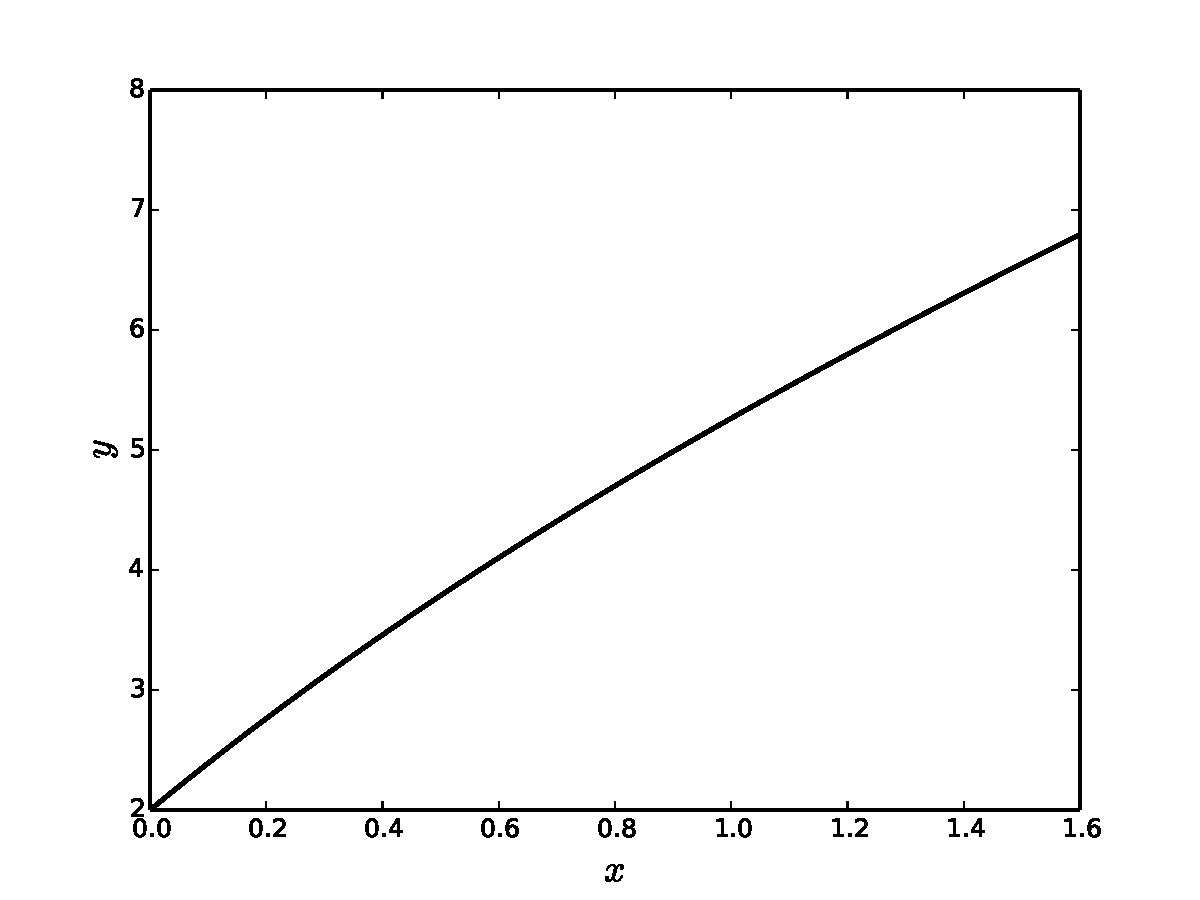
\includegraphics[width=\textwidth]{Example1.pdf}
% \caption{The solution of $y'(t) = 6+2t-y$, $y(0) = 2$, on the interval $[0,1.6]$, using the solver \li{dopri5} from \li{scipy.integrate}.}
% \label{sir:example1}
% \end{figure}
% 
% 
% \begin{problem}
% Using \li{dopri5}, solve the IVP
% \begin{align*}
% 5y''' + y'+2y &= 0, \,\, 0 \leq x \leq 16,\\
% y(0) &=0,\\
% y'(0) &= 1,\\
% y''(0) &= -2.
% \end{align*}
% \end{problem}
% 
% Another good ode solver to try is \li{odeint}, also in \li{scipy.integrate}. \li{odeint} is a Python wrapping for the function \li{lsoda} from the Fortran library \li{odepack}. One of the nice features of \li{lsoda} is that it automatically switches between stiff and nonstiff solvers depending on the behavior of the problem. 
% 
% 
% \section*{The SIR Model}
The SIR model describes the spread of an epidemic throughout a large population. It does this by describing the movement of the population through three phases of the disease: those individuals who are Susceptible, those who are Infectious, and those who have been Removed from the disease. Those individuals in the Removed class have either died, or have recovered from the disease and are now immune to it. If the outbreak occurs over a short period of time, we may reasonably assume that the total population is fixed, so that $S'(t) + I'(t) + R'(t) = 0$.  We may also assume that $S(t) + I(t) + R(t) = 1$, so that $S(t)$ represents the \textit{fraction} of the population that is susceptible, etc. 

Individuals may move from one class to another as described by the flow 
\[S \to I \to R.\] Let us consider the transition rate between $S$ and $I $. Let $\beta$ represent the average number of contacts made per day that could spread the disease. The proportion of these contacts that are with a susceptible individual is $S(t)$. Thus, one infectious individual will on average infect $\beta S(t)$ others per day. Let $N$ represent the total population size. Then we obtain the differential equation
 \[\frac{d}{dt}(S(t) N) = -\beta S(t) (I(t) N).\]
 
 Now consider the transition rate between $I$ and $R$. We assume that there is a fixed proportion $\gamma$ of the infectious group who will recover on a given day, so that 
 \[\frac{d}{dt}R(t) = -\gamma I(t).\]
 Note that the proportion who will recover on a given day is the reciprocal of the average length of time spent in the infectious phase. 
 
 Since we have $I'(t) = - S'(t) - R'(t)$, the  differential equations are given by
\begin{align*}
\frac{dS}{dt} &=-\beta IS ,\\
\frac{dI}{dt} &= \beta I S-\gamma I, \\
\frac{dR}{dt} &=\gamma I.
\end{align*}


\begin{problem}
Solve the IVP
\begin{align*}
\frac{dS}{dt} &=-\frac{1}{2} IS ,\\
\frac{dI}{dt} &= \frac{1}{2} I S-\frac{1}{4} I, \\
\frac{dR}{dt} &=\frac{1}{4} I,\\
S(0) &= 1-6.25\cdot10^{-7},\\
I(0) &= 6.25\cdot10^{-7},\\
R(0) &=0,
\end{align*}
on the interval $[0,100]$. \label{prob_sir1}
\end{problem}

\begin{figure}[ht]
\centering
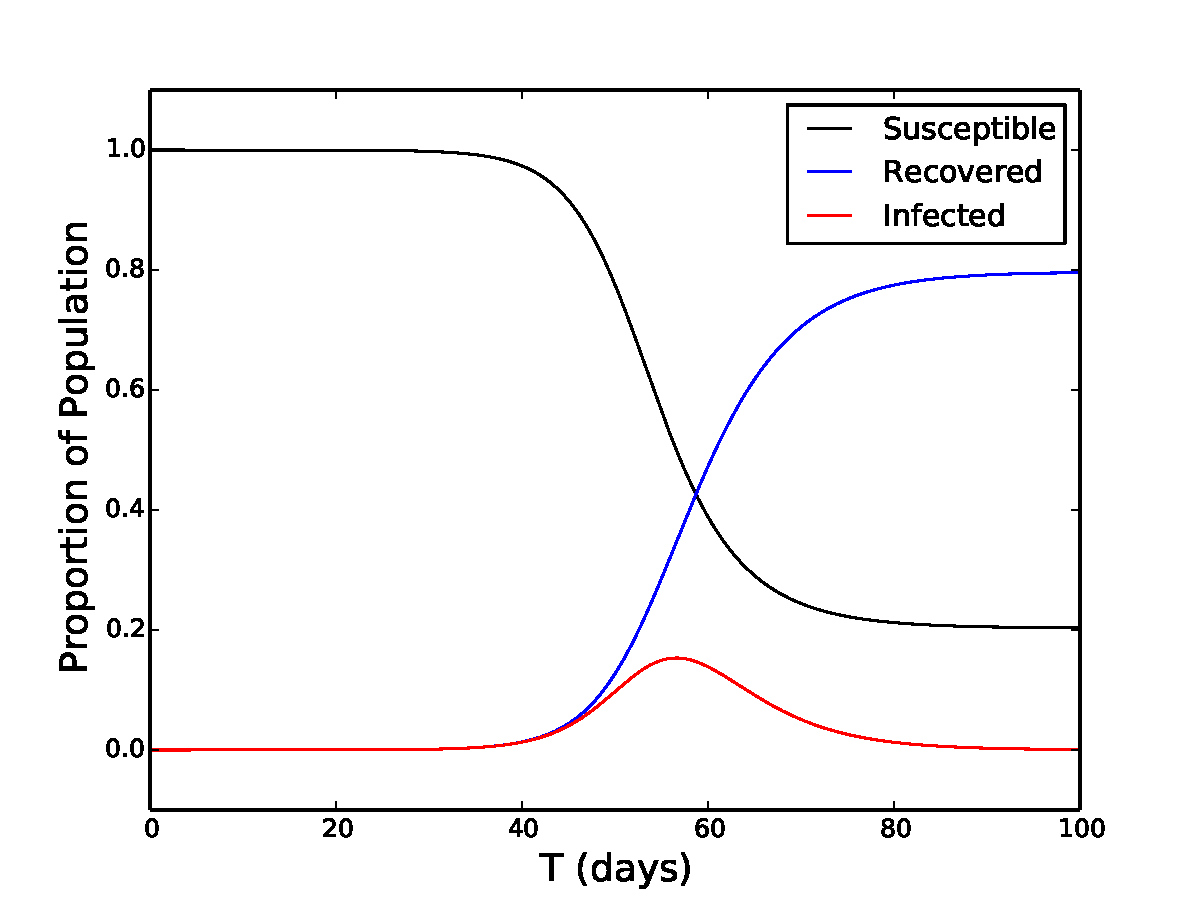
\includegraphics[width=\textwidth]{SIR1.pdf}
\caption{Solution to Problem (\ref{prob_sir1}) }
\label{sir1}
\end{figure}

\begin{problem}
Suppose that, in a city of approximately three million, five have recently entered the city carrying a certain disease. (Suppose they have just entered the infectious state.)

Each of those individuals has a contact each day that will spread the disease, and average of three days is spent in the infectious state. Find the solution of the corresponding SIR equations for the next fifty days. 

Assume for simplicity that those who are in the infectious state either cannot go to work or are unproductive, etc. At the peak of the infection, how many in the city will still be able to work? 
Answer the same question if instead of three days, an average of seven days is spent in the infectious state.
\end{problem}


\begin{problem}
Suppose that, in a city of approximately three million, five have recently entered the city carrying a certain disease. (Suppose they have just entered the infectious state.) 

Each of those individuals will make three contacts every ten days that will spread the disease, and average of four days is spent in the infectious state. Find the solution of the corresponding SIR equations. Choose an appropriate time interval and plot your results.
\end{problem}


\section*{Variations on the SIR Model}


SIS Models describe diseases where individuals who have recovered from the disease do not gain 
any lasting immunity. There are only two compartments in this model: those who are Susceptible, and 
those who are infectious.

The basic equations are given by 
\begin{align*}
\frac{dS}{dt} &=-\beta I S + \gamma I ,\\
\frac{dI}{dt} &= \beta I S-\gamma I.
\end{align*}


If we add to our basic SIR model to account for the death rate and an equal birth rate, the equations become
\begin{align*}
\frac{dS}{dt} &=\mu(1 -S) - \beta I S,\\
\frac{dI}{dt} &= \beta I S - (\gamma + \mu)I, \\
\frac{dR}{dt} &= \gamma I - \mu R.
\end{align*}

SIRS model takes the previous model, and allows the transfer of individuals from the recovered/removed class to rejoin the susceptible class. 
\begin{align*}
\frac{dS}{dt} &= fR + \mu(1 -S) - \beta I S,\\
\frac{dI}{dt} &= \beta I S - (\gamma + \mu)I, \\
\frac{dR}{dt} &= -fR + \gamma I - \mu R.
\end{align*}

The next exercise uses a variation of the basic SIR model to describe the spread of measles. 
It assumes that the rate at which measles is contracted depends on the season, i.e. the rate is periodic. That means that likely the spread of measles is periodic, and can be described as the solution of a boundary value problem (BVP).
Many-industry grade BVP solvers have been written in Fortran. One of these, \li{bvp_solver}, has been wrapped in Python as a scikit. The code below demonstrates how to use \li{bvp_solver} to solve the BVP
\begin{align*}
	\epsilon y'' + yy' - y &= 0, \quad y(-1) = 1, \quad y(1) = -1/3.
\end{align*}

\begin{lstlisting}
import numpy as np
from scikits import bvp_solver
import matplotlib.pyplot as plt

epsilon, lbc, rbc = .1, 1., -1/3.

def ode(x , y):
	return np.array([y[1] , (1./epsilon)*(y[0]- y[0]*y[1]) ]) 

def bcs(ya,yb): 				 # Boundary conditions
	BCa = np.array([ya[0] - lbc])# 1 Boundary condition on the left
	BCb = np.array([yb[0] - rbc])# 1 Boundary condition on the right
	return BCa, BCb

problem = bvp_solver.ProblemDefinition(num_ODE = 2,
                                     num_parameters = 0,
                                     num_left_boundary_conditions=1,
                                     boundary_points = (-1, 1),
                                     function = ode,
                                     boundary_conditions = bcs)
solution = bvp_solver.solve(problem,
                            solution_guess = (-1/.3,-4./3))

A = np.linspace(-1.,1., 200); T = solution(A)
plt.plot(A, T[0,:],'-k',linewidth=2.)
plt.show()

\end{lstlisting}

\begin{problem}
SEIR models are another variation of the basic SIR model. Basically they added another compartment, called the exposed or latency phase, to the basic compartments Susceptible, Infectious, and Recovered. 

An SEIR model is used to describe the spread of measles (see \footnote{Numerical Solution of Boundary Value Problems for Ordinary Differential Equations, by Aescher, Mattheij, and Russell} ). The rate at which susceptible individuals may contract measles is seasonal, and corresponds to a periodic function $\beta(t) = \beta_0(1 + \beta_1 \cos{2\pi t})$. Parameters $\mu$ and $\lambda$ represent the birth rate of the population and the latency period of measles, respectively. $\eta$ represents the infectious period before an individual moves from the Infectious class to the Recovered class. After recovery an individual remains immune. The boundary value problem is given by
\begin{align*}
\left[\begin{array}{c}S \\ E \\ I\end{array}\right]' &= \left[\begin{array}{c}\mu - \beta(t) S I \\\beta(t) SI - E/\lambda \\E/\lambda - I/\eta\end{array}\right],\\
S(0) &= S(1),\\
E(0) &= E(1),\\
I(0) &= I(1).
% \left[\begin{array}{c}S \\E \\I\end{array}\right](0) &= \left[\begin{array}{c}S \\E \\I\end{array}\right](1).
\end{align*}
Solve this BVP with parameters  $\beta_1 = 1,$ $\beta_0 = 1575,$ $\eta = 0.01,$ $\lambda = .0279,$ and $\mu = .02.$ 

Hint: \li{bvp_solver} requires \emph{separated boundary conditions}. In other words, each equation in the set of boundary conditions can only include values at one end of the interval. 
To deal with this, let $C = [C_1, C_2, C_3]$, and add the equation 
\[C' = 0\]
to the system of odes given above. Then the boundary conditions can be separated using the following trick: 
\begin{align*}
	\begin{pmatrix}C_1(0) \\C_2(0) \\ C_3(0) \end{pmatrix} &= \begin{pmatrix}S(0) \\E(0) \\ I(0) \end{pmatrix}, \quad 	\begin{pmatrix}C_1(1) \\C_2(1) \\ C_3(1) \end{pmatrix} = \begin{pmatrix}S(1) \\E(1) \\ I(1) \end{pmatrix}.
\end{align*}


\label{sir_measles}
\end{problem}

\begin{figure}[ht]
\centering
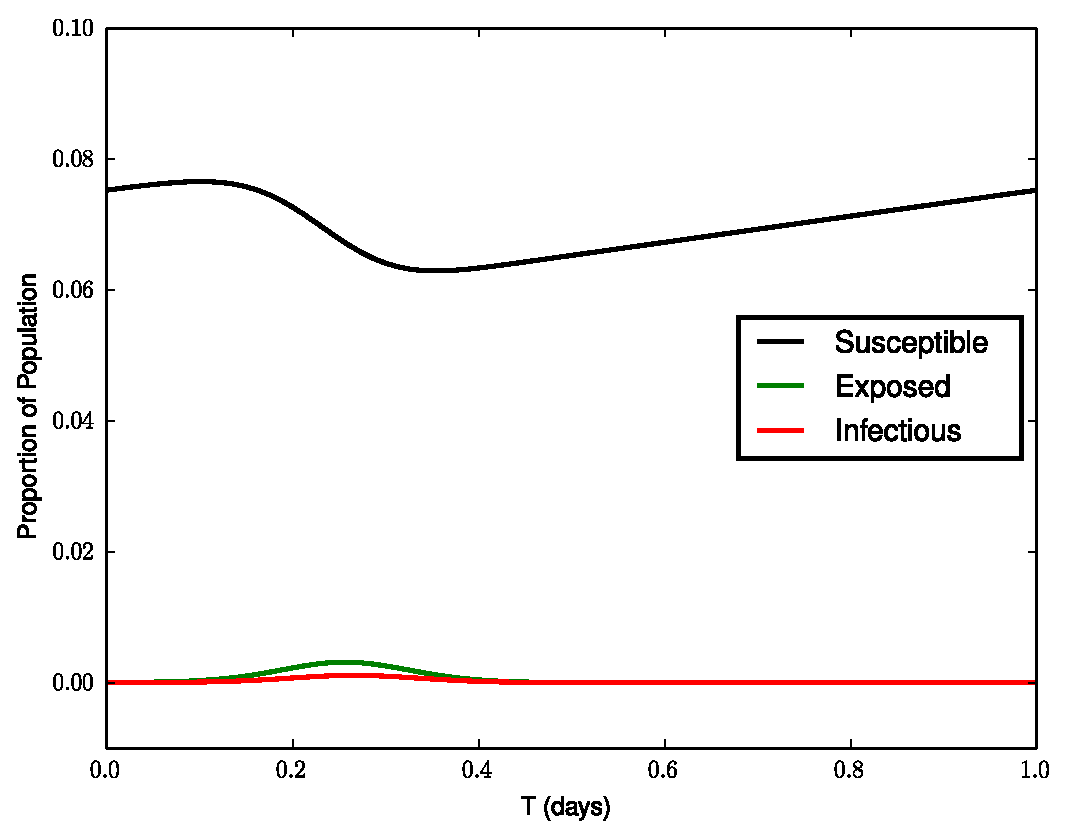
\includegraphics[width=\textwidth]{measles.pdf}
\caption{Solution to Problem (\ref{sir_measles}) }
\label{sir4}
\end{figure}






